
\section{Definici�n del Problema}
\begin{frame}{Definici�n del Problema}

\framesubtitle{Reconocimiento de Actividades Humanas (HAR)}
\begin{center}
Determinar la actividad o comportamiento de una (o m�s) persona(s)
a trav�s de datos prove�dos por sensores situados en el entorno.
\par\end{center}

\end{frame}
%
\begin{frame}{Definici�n del Problema}

\framesubtitle{Que es HAR}
\begin{itemize}
\item Investigaci�n en m�ltiples �reas
\begin{itemize}
\item Capturar movimientos
\item Interacci�n con el entorno
\item Aprender e inferir
\end{itemize}
\end{itemize}
\begin{center}
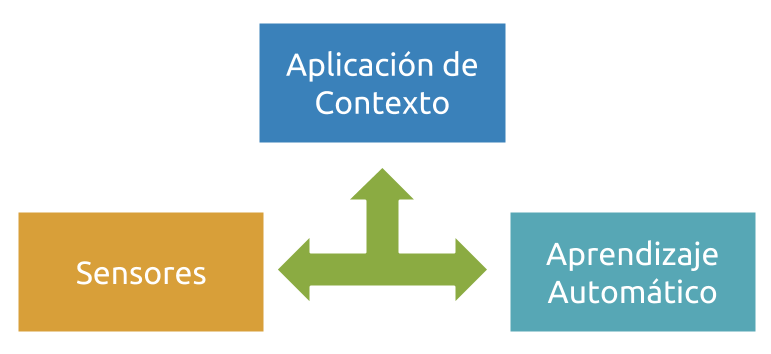
\includegraphics[width=8cm]{intro/graphics/areas}
\par\end{center}
\end{frame}

